\documentclass[../main.tex]{subfiles}

\begin{document}

Suppose you drive from city A to city B which is 200km's in 2 hours. Your average speed is 100km/h. Even if you did not travel constant speed. There is at least one instant where  your speed was exactly 100km/h. This is called \textbf{mean value theorem}.

\begin{figure}[htbp]
    \centering
    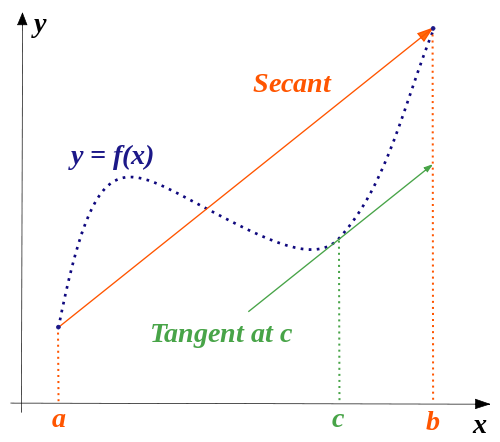
\includegraphics[scale=.4]{mean-val-thm.png}
    \caption{Mean Value Theorem says that the slope of the secant line joining two points on the graph of of $f(x)$ is equal to the slope of the tangent line at some point $x=c$ between $a$ and $b$. from Wikipedia.}
\end{figure}

\begin{theorem}[The Mean-Value Theorem]
    Suppose that $f$ is cts on the interval $[a, b]$ and that it is differentiable on the open inteval $(a, b)$. Then there exists a point $c$ in the open interval $(a, b)$ s.t.
    \[
        \frac{f(b) - f(a)}{b - a} = f'(c).
    \]
\end{theorem}

Let $f(t)$ denote the distance from city A. Then $f(0) = 0$ and $f(2) = 200$. MVT says there is a time $t = c$ s.t. $f'(c) = 100$.

\begin{figure}[htbp]
    \centering
    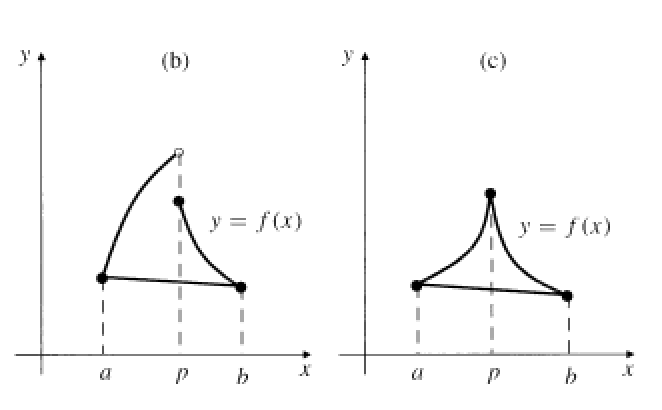
\includegraphics[scale=1]{mean-val-thm2}
    \caption{Functions that fail to satisfy the Mean Value Theorem. (b) $f$ is discts at $p$, (c) $f$ is not differentiable at $p$.}
\end{figure}

If the assumptions of the Mean Value Theorem are satisfied:
\begin{itemize}
    \item We don't know how to find $c$.
    \item We don't know how many different $c$ can be found satisfying MVT (there is at least one).
\end{itemize}
In short, MVT is an \textit{existence theorem} like Intermediate Value Theorem and Min-Max Theorem.

\begin{example}
    Show that $\sin x < x$ for all $x>0$.
\end{example}
\begin{solution}
    For $x > 2\pi$ done. For $0<x<2\pi$, use the MVT and $\cos c < 1$.
\end{solution}

\begin{example}
    Show that $\sqrt{1+x} < 1 + \frac{x}{2}$ for all $x>0$.
\end{example}
\begin{solution}
    Let $f(x) = \sqrt{1+x}$. Then $f'(c) < \frac{1}{2}$ for $c>0$. Use MVT.
\end{solution}

Suppose $f$ is defined on an interval $I$. If $f(x_2) > f(x_1)$ for all $x_1, x_2$ in $I$ s.t. $x_2 > x_1$ then we say $f$ is \textbf{increasing} on $I$. Similarly define \textbf{decreasing, non-increasing, non-decreasing} on $I$.

\begin{theorem}
    Suppose $f$ is differentiable on an open interval $I$.
    \begin{itemize}
        \item If $f'(x)>0$ for all $x \in I$ then $f$ is increasing on $I$.
        \item If $f'(x) \geq 0$ for all $x \in I$ then $f$ is nondecreasing on $I$.
    \end{itemize}
    Similar statements hold for decreasing and nonincreasing functions.
\end{theorem}
\begin{proof}
    Prove first statement. Let $x_2 > x_1$ in $I$. Use MVT, $f(x_2) - f(x_1) = f'(c) (x_2 - x_1) > 0$.
\end{proof}

\begin{example}
    On what intervals is $f(x) = x^3 - 12 x + 1$ increasing or decreasing?
\end{example}
\begin{solution}
    $f'(x) = 3(x-2)(x+2)$. So $f$ is decreasing on $(-2, 2)$ and increasing otherwise.
    \begin{figure}[H]
        \centering
        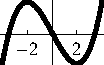
\includegraphics[scale=1]{mvt-ex.pdf}
        \caption{Graph of $f(x) = x^3 - 12 x + 1$.}
    \end{figure}
\end{solution}

We know that if $f$ is a constant function then its derivative is zero. The converse is also true.
\begin{theorem}
    If $f$ is cts on the interval $I$ and $f'(x) = 0$ at every $x$ in $I$ then $f(x) = C$, a constant on $I$.
\end{theorem}
\begin{proof}
    Choose $x_0$ in $I$. Let $C = f(x_0)$. If $x$ is any other point in $I$ then by MVT, $f(x) - f(x_0) = f'(c) (x-x_0) = 0$.
\end{proof}
\end{document}